\RequirePackage{luatex85}
\documentclass[tikz]{standalone}
% Default preamble
\usepackage{pgfplots}
\pgfplotsset{compat=newest}

\begin{document}
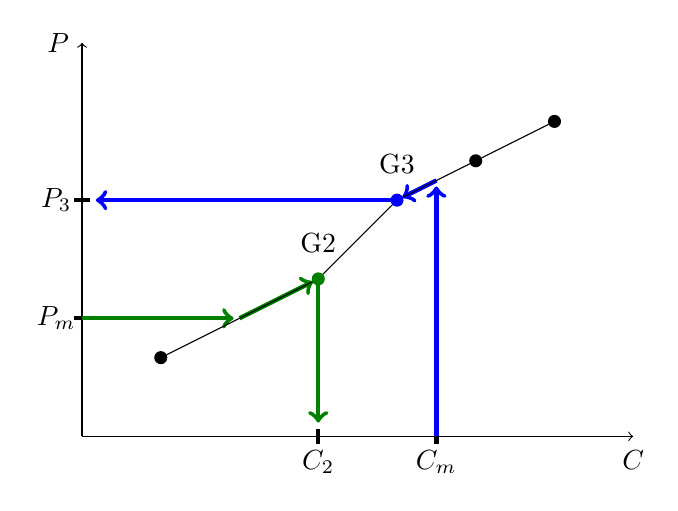
\begin{tikzpicture}
\tikzset{point/.style={circle, fill=black, draw=black, inner sep=1pt, minimum size=1ex}}
\tikzset{b/.style={rectangle, fill=black, draw=black, inner sep=1pt, minimum size=1ex}}
\draw[->] (0,0) -- (7,0) node [pos=1, yshift=-2ex,, fill=white, inner sep=2px] {$C$};
\draw[->] (0,0) -- (0,5) node [pos=1, xshift=-2ex, fill=white, inner sep=2px] {$P$};

\node[point] at (1,1) (p1) {};
\node[point, green!50!black] at (3,2) (p2) {}; \node[above of=p2, node distance=3ex] {G2};
\node[point, blue] at (4,3) (p3) {};
\node[above of=p3, node distance=3ex] {G3};
\node[point] at (5,3.5) (p4) {};
\node[point] at (6,4) (p5) {};

\draw[ultra thick] (4.5, 0.1) -- (4.5, -0.1) node [pos=1, yshift=-1.5ex] {$C_m$};
\draw[->, ultra thick, shorten >=0.5ex, color=blue] (4.5, 0) -- (4.5, 3.25);
\draw[->, ultra thick,shorten >=0.5ex, color=blue] (4.5, 3.25) -- (4, 3);
\draw[->, ultra thick,shorten >=0.5ex, color=blue] (4, 3) -- (0.1, 3);
\draw[ultra thick] (0.1, 3) -- (-0.1, 3) node [pos=1, xshift=-1.5ex] {$P_3$};

\draw[ultra thick] (0.1, 1.5) -- (-0.1, 1.5) node [pos=1, xshift=-1.5ex] {$P_m$};
\draw[->, shorten >=0.5ex,
ultra thick,color=green!50!black] (0, 1.5) -- (2, 1.5);
\draw[->, shorten >=0.5ex, ultra thick, color=green!50!black] (2, 1.5) -- (3, 2);
\draw[->, shorten >=0.5ex,
ultra thick,color=green!50!black] (3, 2) -- (3, 0.1);
\draw[ultra thick] (3, 0.1) -- (3,-0.1) node [pos=1, yshift=-1.5ex] {$C_2$};

\draw[-] (p1) -- (p2) -- (p3) -- (p4) -- (p5);
\end{tikzpicture}
\end{document}
